% Chapter Template

\chapter{Ensayos y resultados} % Main chapter title
En esta sección se presentan los resultados obtenidos del desarrollo de hardware y software. Se analiza el cumplimiento de requisitos de desempeño impuestos por el cliente y finalmente, se exponen resultados de un ensayo \textit{end-to-end} con la red LoRaWAN.\\
\label{Chapter4} % Change X to a consecutive number; for referencing this chapter elsewhere, use \ref{ChapterX}
%----------------------------------------------------------------------------------------
%	SECTION 1
%----------------------------------------------------------------------------------------
\section{Circuito impreso desarrollado}
\label{sec:pruebasHW}
Gracias al desarrollo temprano de la primera placa prototipo de la figura \ref{fig:placaprototipo}, se realizaron las primeras validaciones de diseño de circuitos y selección de componentes para las diferentes etapas del hardware presentadas en \ref{seccion_hardware}.\\
Disponer de una placa con la mayoría de las etapas ya montadas, soldadas y depuradas, ayudó a reducir fallas eléctricas tales como falsos contactos que ocurrieron al usar protoboards.\\
% TODO: \usepackage{graphicx} required
\begin{figure}[h]
	\centering
	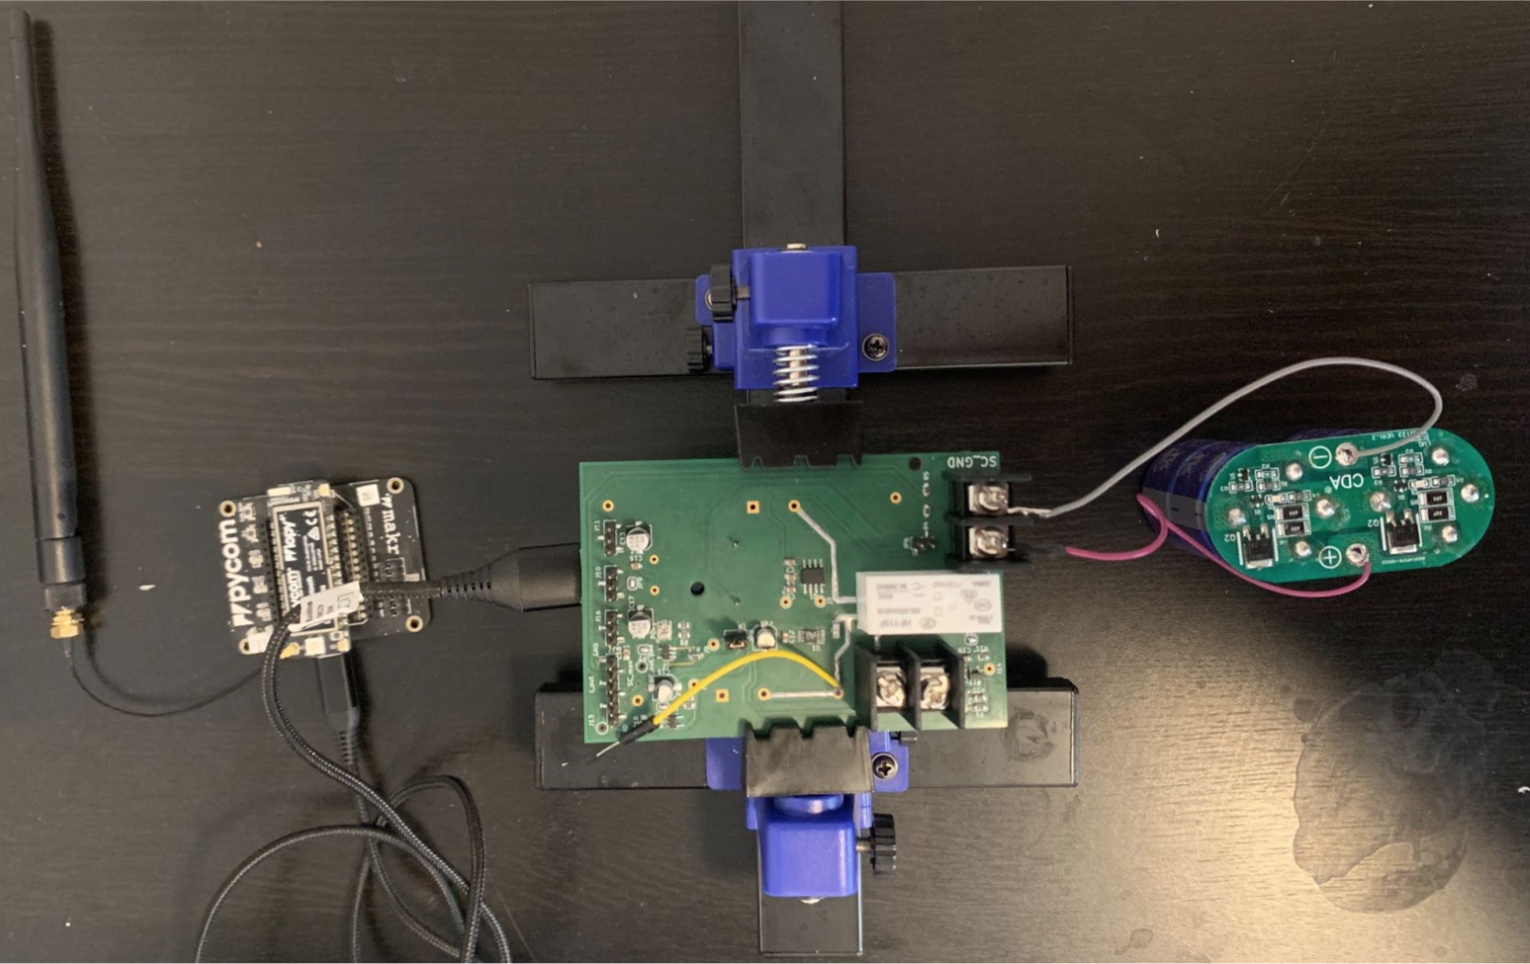
\includegraphics[width=0.7\linewidth]{Figures/placa_prototipo}
	\caption{Placa prototipo desarrollada para validación de diseños.}
	\label{fig:placaprototipo}
\end{figure}\\
Una vez validados los diseños mediante la primera placa, se desarrolló la placa final presentada en las figuras \ref{fig:pcbfinaltop} y \ref{fig:pcbfinabottom}. Esta, a diferencia de la primera versi\'{o}n integra toda las etapas en un único circuito impreso.\\
% TODO: \usepackage{graphicx} required
\begin{figure}[h!]
	\centering
	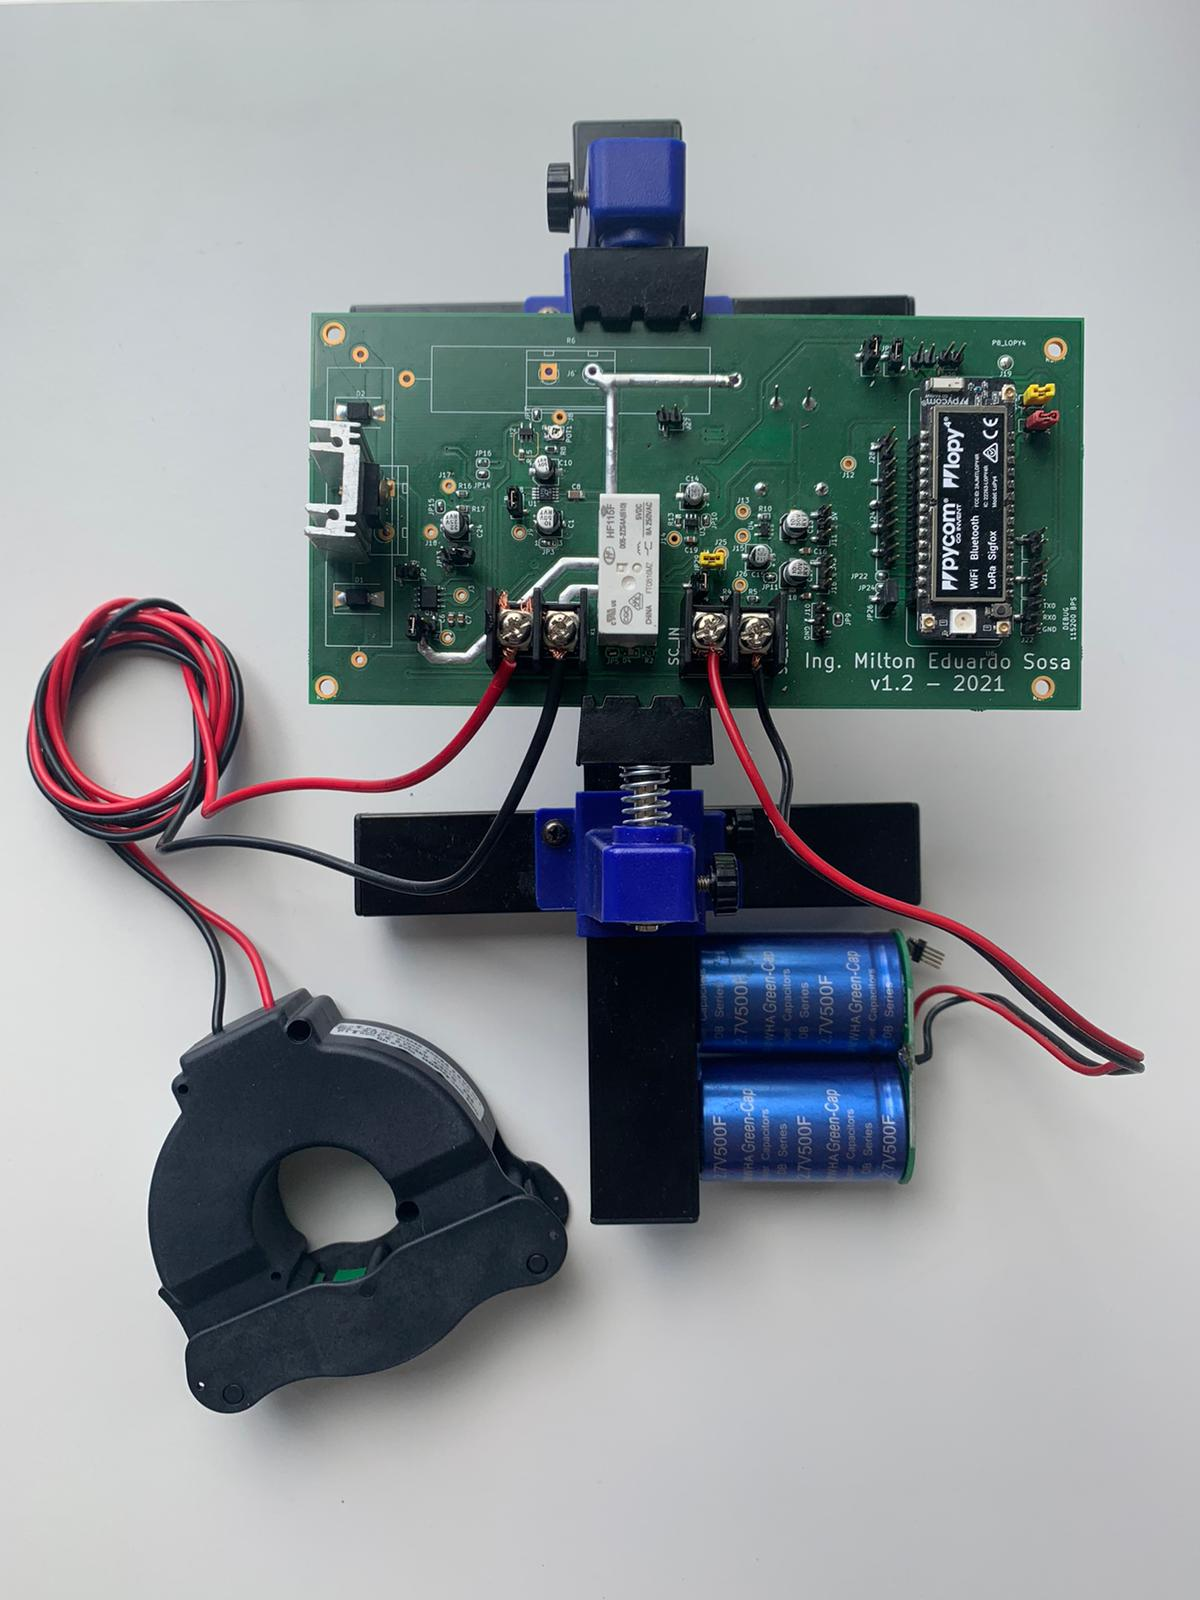
\includegraphics[width=0.9\linewidth]{Figures/banco_prueba_e2e_2}
	\caption{Lado TOP del circuito impreso final integrando todas las etapas.}
	\label{fig:pcbfinaltop}
\end{figure}\\
% TODO: \usepackage{graphicx} required
\begin{figure}[h!]
	\centering
	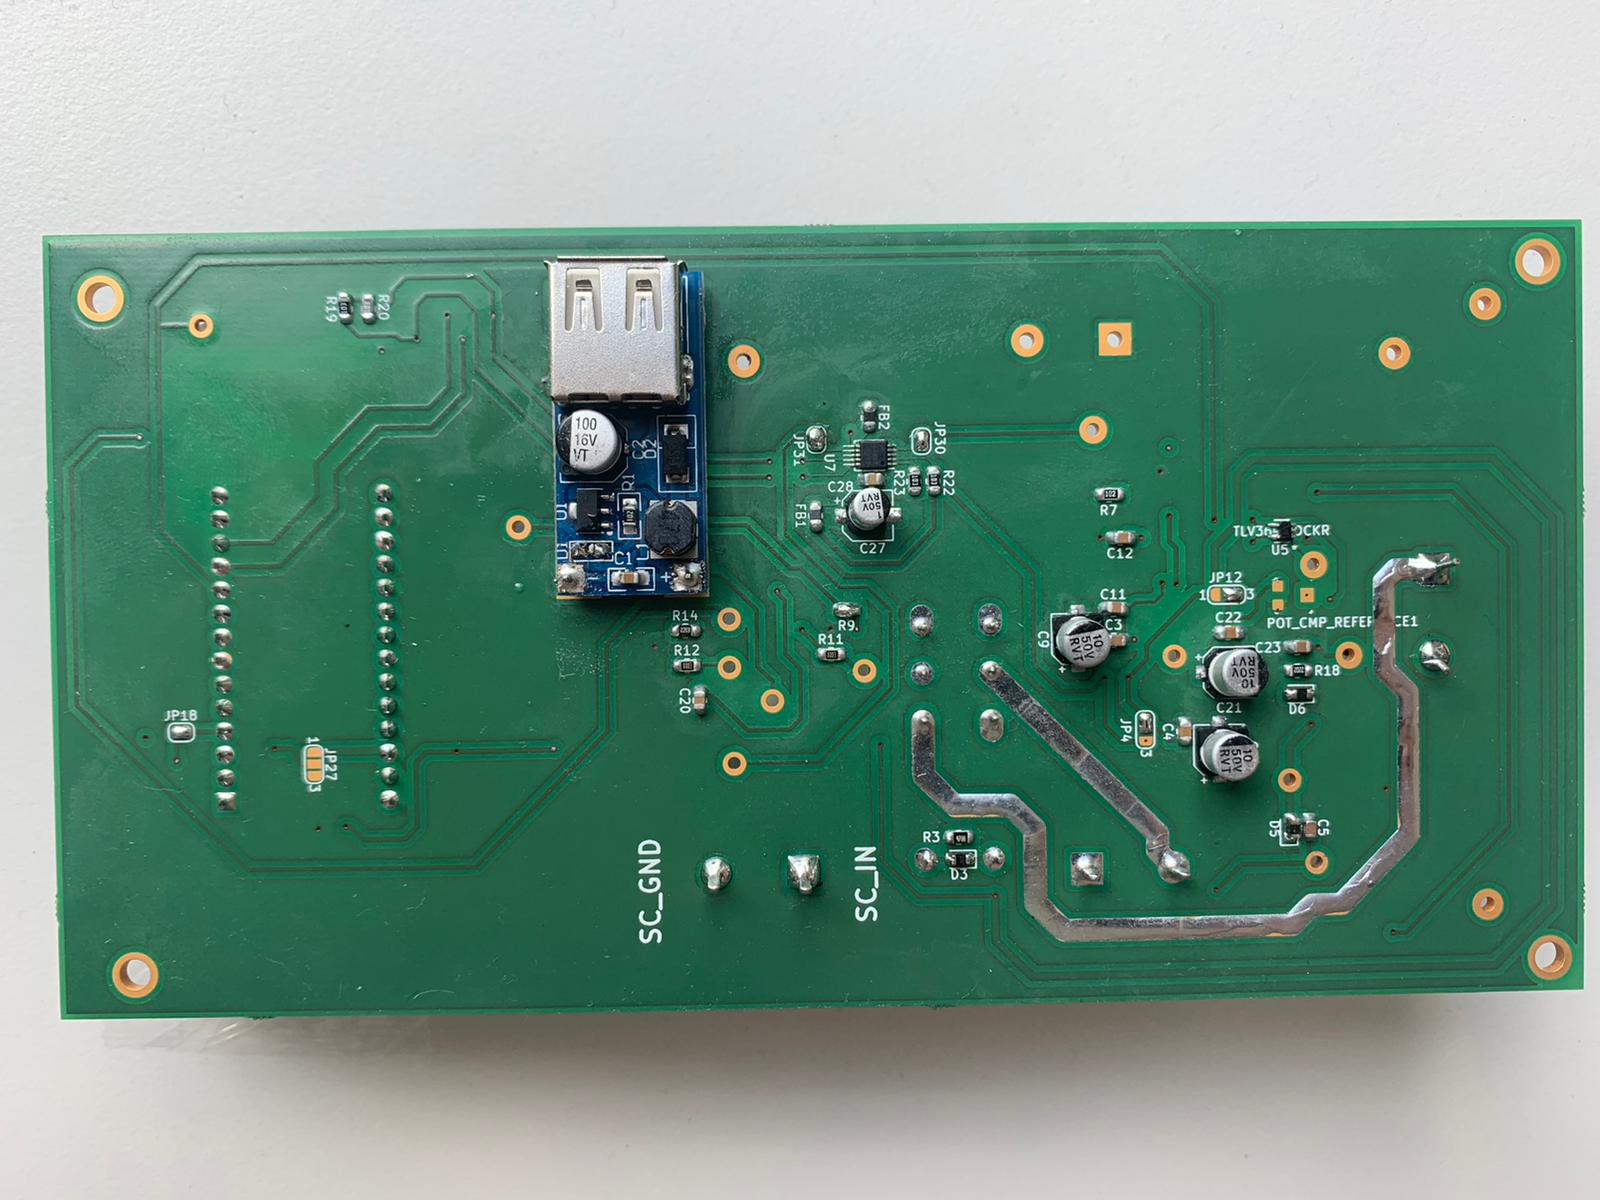
\includegraphics[width=0.8\linewidth]{Figures/pcb_fina_bottom}
	\caption{Lado BOTTOM del circuito impreso final que alberga todas las etapas.}
	\label{fig:pcbfinabottom}
\end{figure}

\section{Ensayos de laboratorio}
Debido a la imposibilidad de acceder a un laboratorio con instrumental de precisión, las mediciones tomadas en los ensayos se realizaron por partes y en diferentes turnos.\\
Como instrumento de medición se contó únicamente con un multímetro de la marca HoldPeak modelo HP-770d \citep{hp770d}.\\
Un generador de senales de la marca \textit{Feel Tech} modelo FY6900 se empleo para generar
\subsection{Consumo en modo ahorro de energia o \textit{deep sleep}}
El instrumento elegido tiene un rango de medición de corriente que permite medir desde los uA hasta 400 mA. Este rango pareció suficiente para la medición de corriente en ambos estados sin la necesidad de cambiar de escala. Sin embargo, en las primeras rondas de medición se advirtió que al salir del modo ahorro de energía y transmitir, la corriente consumida por el hardware generó una tensión de burden en el instrumento que causó que el microcontrolador se reseteara por desvanecimiento (Brown Out Reset-).\\
Como solución para el ensayo de consumo en \textit{deep sleep}, se grabó sobre la LoPy4 una versión de firmware que llevó al hardware al modo ahorro de energía apenas se energizó por al menos 10 minutos. Un tiempo suficiente para registrar el consumo de corriente en este modo.\\
Para la medición de consumo durante la transmisión, se programó la versión final de firmware. Para sortear el problema de reseteo por desvanecimiento se utilizó la escala de amperes en conjunto con la función que retiene el pico máximo de la señal.\\
La tabla \ref{tabla_consumos}, expone los resultados promedio para un total de 10 mediciones efectuadas en cada modo.\\
% \usepackage{color}
\begin{table}[h]
	\centering
	\caption{Consumo máximo registrado en los diferentes modos.}
	\begin{tabular}{cc} 
		\hline
		Modo                                                & \begin{tabular}[c]{@{}c@{}}Consumo\\\textcolor[rgb]{0.302,0.318,0.337}{máximo}\end{tabular}  \\ 
		\hline
		\begin{tabular}[c]{@{}c@{}}Deep\\sleep\end{tabular} & 62 uA                                                                                        \\
		Transmisión                                         & 127 mA                                                                                       \\
		\hline
	\end{tabular}\label{tabla_consumos}
\end{table}\\
Si bien el perfil estimado de consumo del hardware es similar al presentado en \ref{fig:ciclodeepsleep}, por falta de equipamiento no se ha podido capturar un oscilograma para graficar su perfil exacto. Tal gráfico se podría haber adquirido con un multímetro de 7 ½ dígitos con la función de almacenamiento.\\
Desenergizar toda la electrónica salvo al microcontrolador, ha reducido el consumo total de la electrónica al orden de los uA. Este valor de consumo registrado, se encuentra debajo de lo requerido por el cliente en \ref{req_deep_sleep} e implica un aumento en la autonomía del acumulador.\\


\subsection{Autonom\'{i}a del supercapacitor}\label{ensayo_autonomia}
Este ensayo tuvo como objetivo principal, verificar el cumplimiento del requerimiento \ref{req_autonomia}.\\
Como única condición inicial, se adoptó que el supercapacitor esté cargado al máximo. Para acelerar el proceso, se lo cargó hasta 5 V mediante una batería de 9 V convencional.\\
Como método de control y registro, se utilizó la tabla de base de datos \ref{fig:tablacorrientesporfase}. El valor de tensión en bornes del supercapacitor se monitoreó de manera constante y se consideró como finalizada la prueba cuando se registró un cese en el almacenamiento de nuevos valores del nodo utilizado.\\
Con un tiempo de ahorro de energia de 5 minutos luego de transmitir, el hardware desarrollado registro una autonomía de 19 horas. Este valor resulta ser un 60\% mayor que el requerido por el cliente. Se estima que el valor podría aumentar aun más anulando el indicador LED de encendido del relay y/o proponiendo un circuito de seleccion de modo utilizando un arreglo de transistores.\\

\subsection{Medidor de valor RMS}\label{ensayo_medidor_rms}
En este ensayo se analizo la linealidad del circuito medidor de valor RMS implementado en \ref{circuito_rms}.\\
El generador FY6900, emulo el valor de la senal generada en bornes del resistor shunt sin la necesidad de utilizar el transformador de corriente ni la carga.\\
Se realizo un barrido de 10 pasos en la amplitud de la onda senoidal a la salida del generador, a su vez se registraron la tension RMS a la entrada del LTC1966 y la tension DC a la salida de la etapa de amplificacion mediante el multimetro. Los valores registrados, se exponen en la tabla VVVV y a partir de \'{e}stos la curva \ref{fig:ensayoinealidadmedidorrms}.\\
% TODO: \usepackage{graphicx} required
\begin{figure}[h]
	\centering
	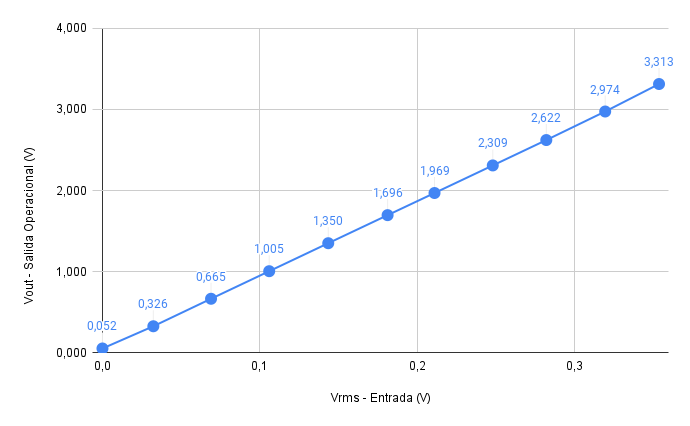
\includegraphics[width=1.0\linewidth]{Figures/ensayo_inealidad_medidor_RMS}
	\caption{Traza para analisis de linealidad del medidor de valor RMS}
	\label{fig:ensayoinealidadmedidorrms}
\end{figure}\\
La traza presentada en la figura \ref{fig:ensayoinealidadmedidorrms}, expone linealidad en todo el rango de medicion. 

\subsection{Circuito detector de cortes}
% TODO: \usepackage{graphicx} required
\begin{figure}
	\centering
	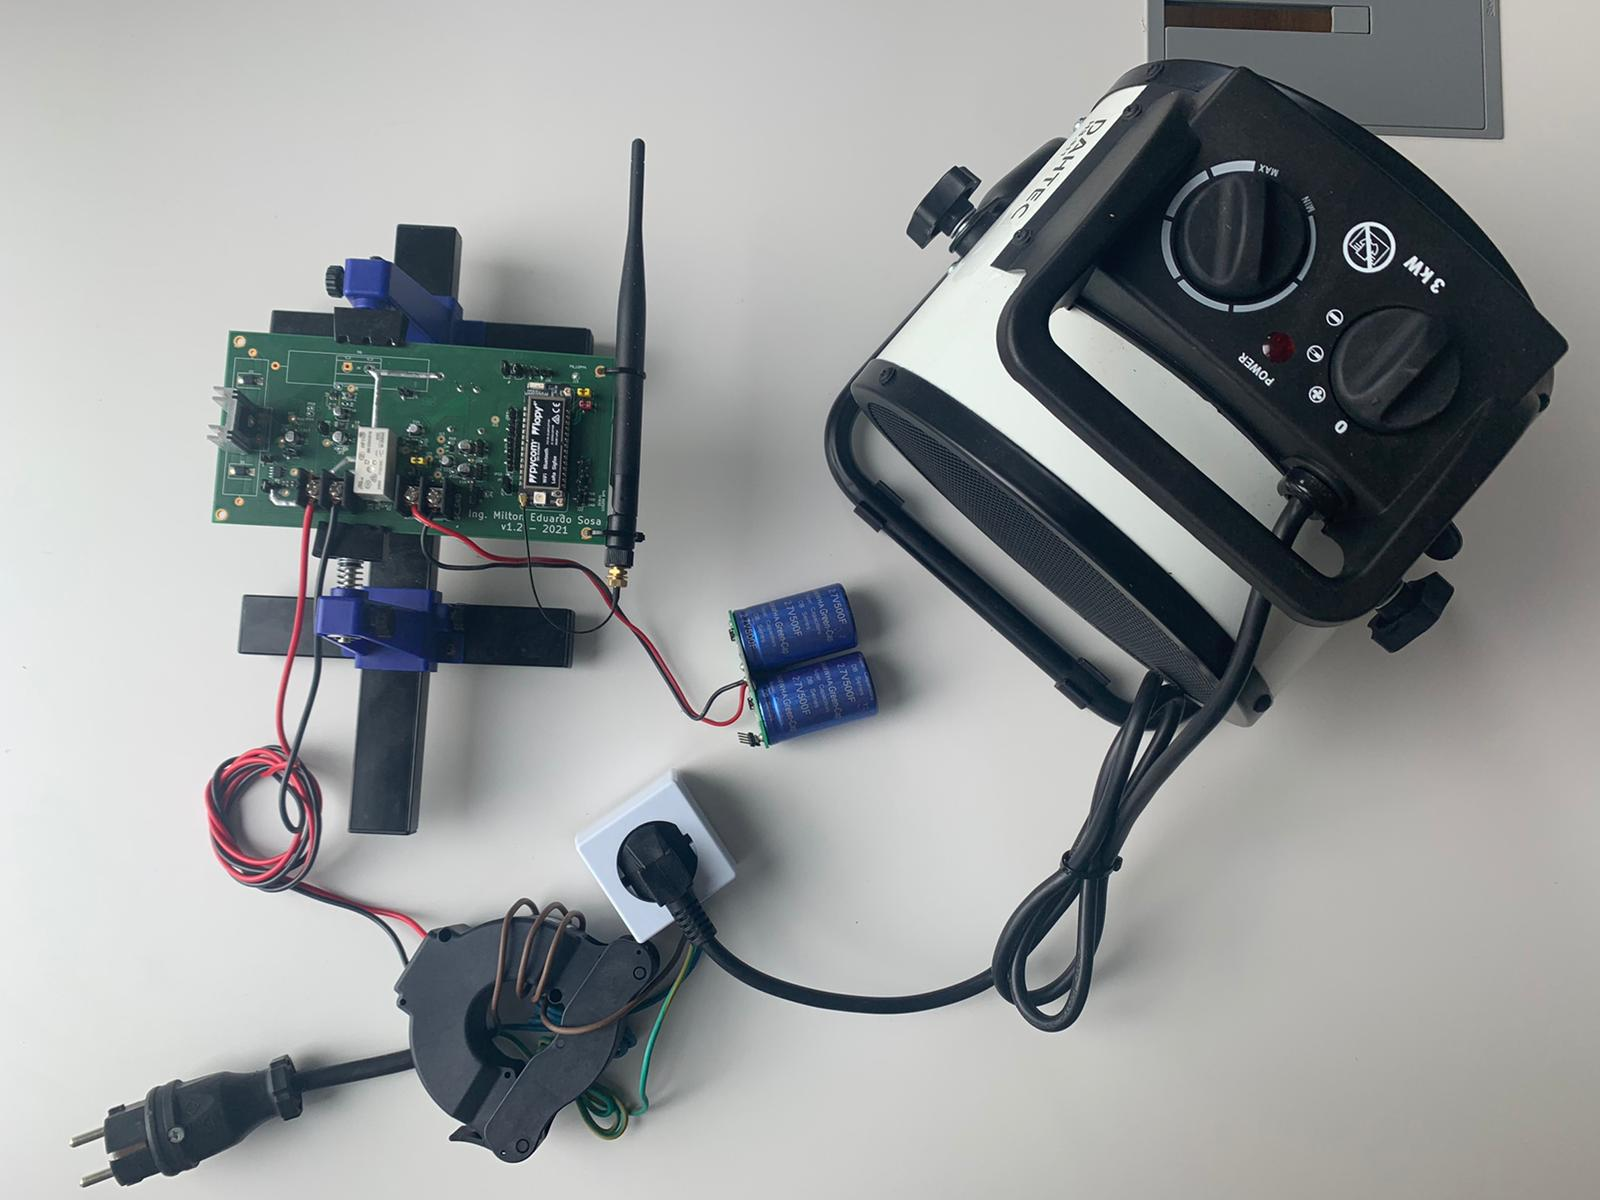
\includegraphics[width=1.0\linewidth]{Figures/banco_prueba_e2e_1}
	\caption{Banco de prueba utilizado en ensayos del circuito detector de corte y end-to-end.}
	\label{fig:bancopruebae2e2}
\end{figure}

\section{Ensayos \textit{end-to-end}}
Con objeto de realizar una prueba final de integracion y funcionamiento de todas las partes, se decidio repetir el ensayo de autonomía y medicion de valor RMS de corriente descritos en \ref{ensayo_autonomia} y \ref{ensayo_medidor_rms} respectivamente, con el agregado de utilizar los paneles de Grafana para la visualizacion de los datos. De este modo, intervinieron todos los m\'{o}dulos de hardware y software desarrollado para este proyecto. Lograndose asi, una verificacion del cumplimiento de los objetivos del proyecto.\\
Es importante mencionar que, si bien el autor conto fisicamente con el hardware en todo momento, no fue asi con los servicios de backend. Esto corrieron sobre una Raspberry Pi 3 B+ localizada en la provincia de Misiones desde el principio del proyecto.\\
Los resultados del ensayo de autonomía expuestos en la figura [CAPTURA DE GRAFANA HISTORICO DE BATERIA], demuestran el correcto funcionamiento y despliegue de informacion historica de la tensión en bornes del supercapacitor.\\
Por su parte en el ensayo de medicion de corriente de la figura \ref{fig:capturahistoricodropdown}, se expone correctamente el barrido de corriente medida por el ciruito expuesto en \ref{circuito_rms}.\\
% TODO: \usepackage{graphicx} required
\begin{figure}[h]
	\centering
	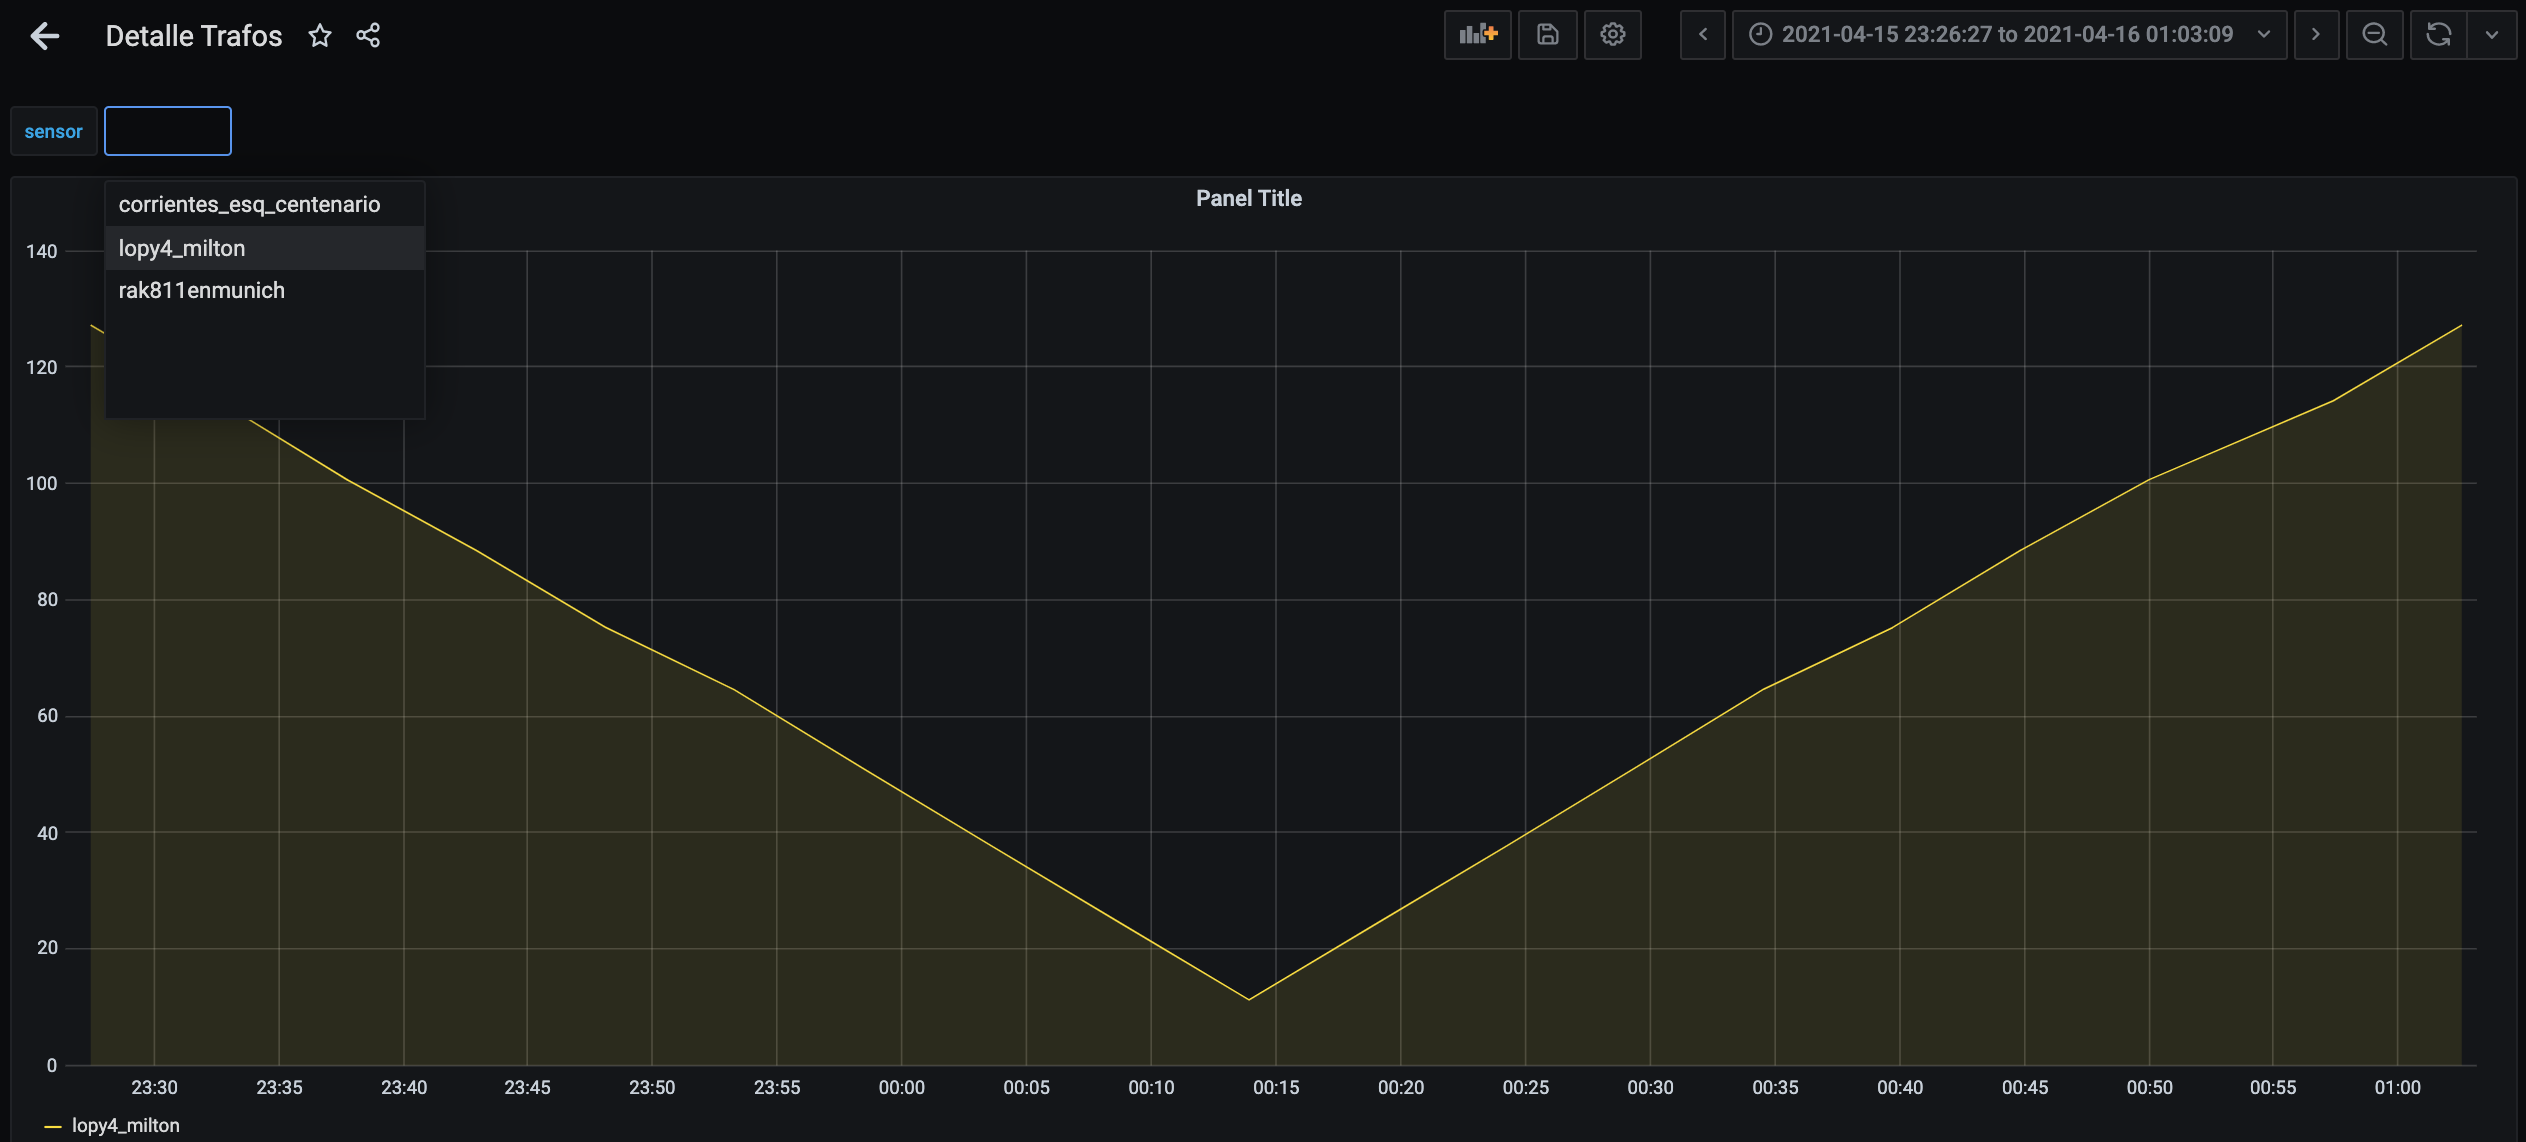
\includegraphics[width=1.0\linewidth]{Figures/captura_historico_dropdown}
	\caption{Ensayo end-to-end de medicion de corriente.}
	\label{fig:capturahistoricodropdown}
\end{figure}\\
El agregado de un \textit{drop down menu} en ambos paneles, permite de manera rapida elegir de que nodo de toda la flota sera la informacion a desplegar en las trazas.\\
Con respecto a la rapidez de propagacion de los datos generados por el hardware hasta aparecer en la interfaz grafica de usuario, el tiempo promedio fue de 5 a 7 segundos.